\documentclass[border=8pt]{standalone}
\usepackage[utf8]{inputenc}
\usepackage{tikz}
\tikzset{
  debole/.style = {rectangle, draw, thick, fill=blue!8, double, double distance=1.5pt, minimum width=28mm, minimum height=16mm, font=\small},
  attr/.style   = {circle, draw, thick, fill=white, minimum size=5pt, inner sep=0},
  pk/.style     = {circle, draw, thick, fill=black, minimum size=5pt, inner sep=0},
  link/.style   = {thick}, et/.style = {font=\footnotesize}
}
\begin{document}
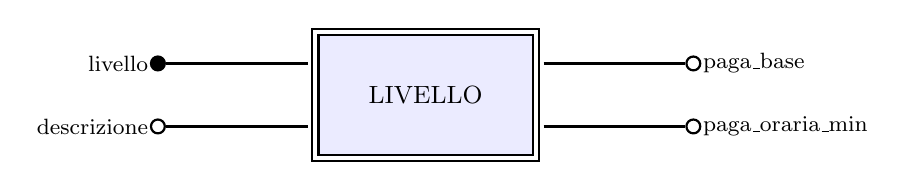
\begin{tikzpicture}
  \node[debole] (E) {LIVELLO};
  \node[pk]   (l)  at (-3.4, 0.4){}; \draw[link] (-1.5, 0.4)--(l);  \node[et,left] at (l)  {livello};
  \node[attr] (d)  at (-3.4,-0.4){}; \draw[link] (-1.5,-0.4)--(d);  \node[et,left] at (d)  {descrizione};
  \node[attr] (pb) at ( 3.4, 0.4){}; \draw[link] ( 1.5, 0.4)--(pb); \node[et,right] at (pb) {paga\_base};
  \node[attr] (po) at ( 3.4,-0.4){}; \draw[link] ( 1.5,-0.4)--(po); \node[et,right] at (po) {paga\_oraria\_min};
\end{tikzpicture}
\end{document}
